\documentclass[a4paper, 12pt]{article}
 
\usepackage[applemac]{inputenc}
\usepackage{graphicx}
\usepackage[french]{babel}
\usepackage[T1]{fontenc}
\usepackage{lmodern}
\usepackage{float}
\usepackage{fullpage}


 
\begin{document}
 
\title{RL : Programming Assignment 4\\Mountain Car}
\author{Mathurin \textsc{Massias} \and Cl�ment \textsc{Nicolle}}
\date{\today} 
 
\maketitle

\section{Position of the problem}

To simulate the inelastic wall, we say that if $x(t+1) = -1.2$ then we calculate $v(t+1)$ with $v(t)$ set to zero. This way, the negative speed is canceled and the car can move to the right with positive speed.\\

Intuitively, the optimal value function would reach a maximum at position $x = 0.6$. On positive positions, it would be huge for high speed, and lower for lower speeds as it won't be enough to reach the top of the mountain. It would also be large for negative positions and speeds, as it is then gaining momentum before to climb the mountain.

\section{Approximate Value Iteration : Fitted-Q iteration} 

At each n draws of couples $(s,a)$, we learn the parameters $\alpha$ with a least-squares regression. With 20 features, 100 iterations of 5000 draws, here is what we obtain for the approximated optimal value function :

\begin{figure}[H]
	\centering
	\noindent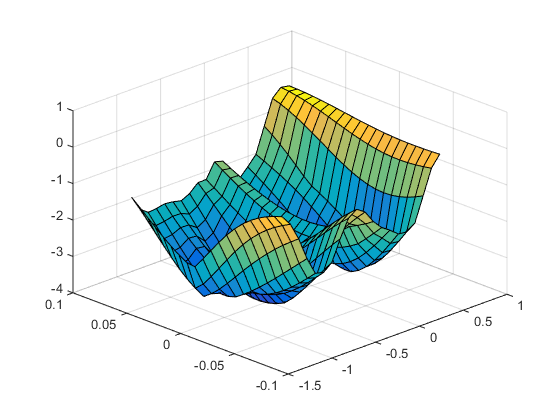
\includegraphics[scale=0.5]{fittedQ-100ep-1000draws-deterministic.png}
	\noindent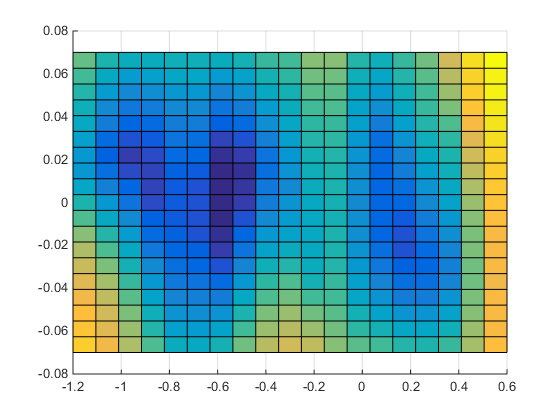
\includegraphics[scale=0.5]{fittedQ-100ep-1000draws-deterministic-levels.png}
	\caption{Left: Approximated optimal value function with fitted-Q for 5000 draws 100 times, in the deterministic case, in 3D - Right : Level values}
\end{figure}

And if we take only 10 features, we get
\begin{figure}[H]
	\centering
	\noindent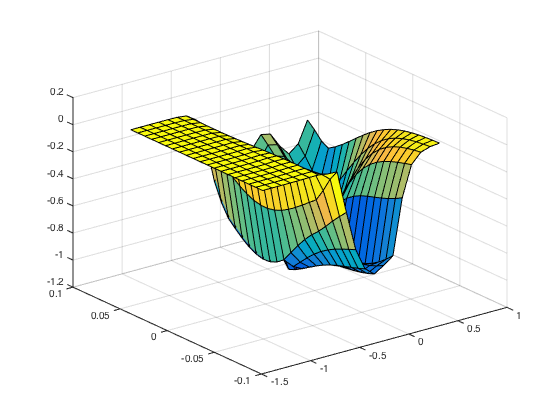
\includegraphics[scale=0.3]{fittedQ-10feat-determ.png}
	\noindent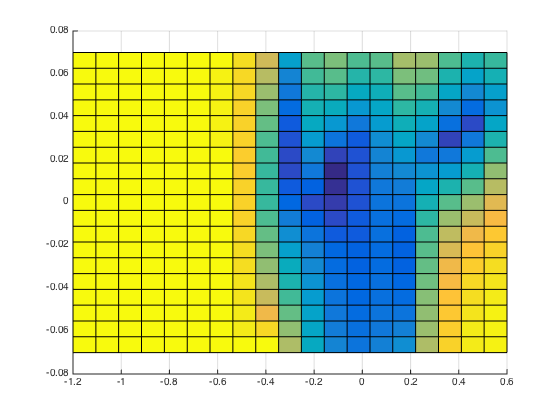
\includegraphics[scale=0.3]{fittedQ-10feat-determ-flat.png}
	\caption{Left: Approximated optimal value function with fitted-Q for 10 features, in the deterministic case, in 3D - Right : Level values}
\end{figure}



\end{document} 